% =====================================================================
% Semana 1 · S1.5 — Fuente real y falla de carga
% Fundamentos de Sistemas Electrónicos Analógicos (Ingeniería Aeroespacial)
% Compilar: pdflatex semana_1_s15_fuente_y_falla.tex  (2 pasadas)
% =====================================================================
\documentclass[aspectratio=169]{beamer}

\usepackage[utf8]{inputenc}
\usepackage[T1]{fontenc}
\usepackage{lmodern}
\usepackage[spanish,es-tabla]{babel}
\usepackage{amsmath,amssymb}
\usepackage{siunitx}
\usepackage{booktabs}
\usepackage{microtype}
\usepackage{circuitikz}

\definecolor{navy}{RGB}{23,54,93}
\definecolor{navysoft}{RGB}{72,101,140}
\definecolor{gold}{RGB}{179,142,62}
\definecolor{ink}{RGB}{44,51,58}
\definecolor{soft}{RGB}{244,241,234}

\usetheme{default}
\setbeamertemplate{navigation symbols}{}
\setbeamertemplate{footline}[frame number]
\setbeamercolor{structure}{fg=navy}
\setbeamercolor{frametitle}{fg=white,bg=navy}
\setbeamercolor{title}{fg=navy}
\setbeamercolor{subtitle}{fg=navysoft}
\setbeamercolor{itemize item}{fg=gold}
\setbeamercolor{itemize subitem}{fg=gold}
\setbeamercolor{block title}{fg=white,bg=navy}
\setbeamercolor{block body}{bg=soft}
\setbeamercolor{example text}{fg=navy}
\setbeamertemplate{itemize item}{\scriptsize\raise1.25pt\hbox{\donotcoloroutermaths$\bullet$}}
\setbeamertemplate{itemize subitem}{\scriptsize\raise1.25pt\hbox{\donotcoloroutermaths$\circ$}}
\setbeamerfont{frametitle}{size=\large,series=\bfseries}

\title[S1.5 · Fuente real]{Fuente real y falla de carga}
\subtitle{S1.5 — Simulaciones y laboratorio de la Semana 1}
\institute{Licenciatura en Ingeniería Aeroespacial\\ UNAM · ENES Unidad Juriquilla}
\author{M. en C. José de Jesús Santana Ramírez}
\date{Semestre 2027-1}

\begin{document}

% ---------------------------------------------------------------------
\begin{frame}[plain]
  \titlepage
\end{frame}

% ---------------------------------------------------------------------
\begin{frame}{Objetivos de la sesión}
  \begin{itemize}
    \item Modelar una \textbf{fuente real} como fuente ideal en serie con una resistencia interna.
    \item Explicar por qué el bus \textbf{cae} al reducir la carga (divisor de carga).
    \item Calcular corriente, tensión de bus y potencia en $R_{interna}$ para $R_L$ de $1\,\text{k}\Omega$ a $1\,\Omega$.
    \item Justificar por qué una fuente real necesita \textbf{límite de corriente}.
  \end{itemize}
  \pause
  \begin{alertblock}{Advertencia de seguridad}
    Este circuito es \textbf{solo para simulación}. No construir los casos de
    $R_L = 10\,\Omega$ o $R_L = 1\,\Omega$ en protoboard: exigen amperios y disipan vatios.
  \end{alertblock}
\end{frame}

% ---------------------------------------------------------------------
\begin{frame}{Teoría 1 · Fuente ideal contra fuente real}
  \begin{columns}[T]
    \begin{column}{0.45\textwidth}
      \resizebox{0.95\linewidth}{!}{%
      \begin{circuitikz}[american voltages, scale=0.9]
        \draw (0,3) to[V, l={$V_{ideal}$}, i=$I$] (0,0);
        \draw (0,3) -- (2.2,3) to[R, l={$R_{int}$}] (4.4,3);
        \draw (4.4,3) -- (5.6,3) to[R, l={$R_{load}$}] (5.6,0);
        \draw (5.6,0) -- (0,0);
        \node[below] at (2.2,0.4) {$V_{bus}$};
      \node[ground] at (0,0) {};
      \end{circuitikz}}
    \end{column}
    \begin{column}{0.5\textwidth}
      \begin{itemize}
        \item Fuente ideal: entrega $V$ constante sin importar la corriente.
        \item Fuente real: $V_{bus} = V_{ideal}\cdot\dfrac{R_L}{R_{int}+R_L}$.
        \item $R_{int}$ modela cables, contactos, batería y electrónica interna.
      \end{itemize}
    \end{column}
  \end{columns}
\end{frame}

% ---------------------------------------------------------------------
\begin{frame}{Teoría 2 · Regulación de carga}
  \begin{itemize}
    \item Con $R_L$ grande (carga ligera), $R_L \gg R_{int}$: $V_{bus} \approx V_{ideal}$.
    \item Con $R_L$ pequeña (carga pesada o falla), la caída en $R_{int}$ domina y el bus se hunde.
  \end{itemize}
  \[
    V_{bus} = V_{ideal}\cdot\frac{R_L}{R_{int}+R_L}
    \qquad\qquad
    I = \frac{V_{ideal}}{R_{int}+R_L}
  \]
  \pause
  \begin{itemize}
    \item La potencia disipada en la resistencia interna: $P_{int} = I^2\,R_{int}$.
    \item En una falla de cortocircuito, $P_{int}$ puede ser enorme: \textbf{se necesita límite de corriente}.
  \end{itemize}
\end{frame}

% ---------------------------------------------------------------------
\begin{frame}{Ejercicio · Enunciado}
  \begin{block}{Fuente de laboratorio modelada con $R_{int}$}
    \centering
    $V_{ideal} = \SI{12}{\volt}$, \quad $R_{int} = \SI{10}{\ohm}$, \quad $R_L$: de $\SI{1}{\kilo\ohm}$ a $\SI{1}{\ohm}$.
  \end{block}
  \begin{center}
    \begin{circuitikz}[american voltages, scale=0.9]
      \draw (0,3) to[V, l={$V_{ideal}=12\,\mathrm{V}$}, i=$I$] (0,0);
      \draw (0,3) -- (2.2,3) to[R, l={$R_{int}=10\,\Omega$}] (4.4,3);
      \draw (4.4,3) -- (5.6,3) to[R, l={$R_{L}$}] (5.6,0);
      \draw (5.6,0) -- (0,0);
    \node[ground] at (0,0) {};
    \end{circuitikz}
  \end{center}
  \textbf{Determinar:} $V_{bus}$, $I$ y $P_{int}$ para $R_L = 1\,\text{k}\Omega$, $100\,\Omega$, $10\,\Omega$ y $1\,\Omega$.
\end{frame}

% ---------------------------------------------------------------------
\begin{frame}{Desarrollo · Paso 1 — Carga ligera: $R_L = \SI{1}{\kilo\ohm}$}
  \[
    I = \frac{12}{10 + 1000} = \SI{11.88}{\milli\ampere}
    \qquad
    V_{bus} = 12\cdot\frac{1000}{1010} = \SI{11.88}{\volt}
  \]
  \[
    P_{int} = I^2\cdot 10 = (11.88\,\text{mA})^2\cdot 10 = \SI{1.41}{\milli\watt}
  \]
  \pause
  \begin{itemize}
    \item La caída es de solo \SI{0.12}{\volt}: la fuente \emph{casi} ideal.
    \item El bus entrega 11.88 V: \SI{99}{\percent} del valor nominal.
  \end{itemize}
\end{frame}

% ---------------------------------------------------------------------
\begin{frame}{Desarrollo · Paso 2 — $R_L = \SI{100}{\ohm}$}
  \[
    I = \frac{12}{10 + 100} = \SI{109.1}{\milli\ampere}
    \qquad
    V_{bus} = 12\cdot\frac{100}{110} = \SI{10.91}{\volt}
  \]
  \[
    P_{int} = (109.1\,\text{mA})^2\cdot 10 = \SI{119}{\milli\watt}
  \]
  \pause
  \begin{itemize}
    \item El bus ya cae \SI{1.09}{\volt}; la corriente se multiplicó $\times 9$.
    \item La resistencia interna empieza a calentarse (119 mW).
  \end{itemize}
\end{frame}

% ---------------------------------------------------------------------
\begin{frame}{Desarrollo · Paso 3 — $R_L = \SI{10}{\ohm}$ (carga pesada)}
  \[
    I = \frac{12}{10 + 10} = \SI{600}{\milli\ampere}
    \qquad
    V_{bus} = 12\cdot\frac{10}{20} = \SI{6.00}{\volt}
  \]
  \[
    P_{int} = (600\,\text{mA})^2\cdot 10 = \SI{3.6}{\watt} \quad (\text{¡el resistor interno disipa 3.6 W!})
  \]
  \pause
  \begin{alertblock}{Observación}
    Con $R_L = R_{int}$ el divisor entrega la \textbf{mitad} de la tensión y la
    mitad de la potencia total se pierde en la fuente. Este caso no se arma en protoboard.
  \end{alertblock}
\end{frame}

% ---------------------------------------------------------------------
\begin{frame}{Desarrollo · Paso 4 — $R_L = \SI{1}{\ohm}$ (falla cercana al corto)}
  \[
    I = \frac{12}{10 + 1} = \SI{1.09}{\ampere}
    \qquad
    V_{bus} = 12\cdot\frac{1}{11} = \SI{1.09}{\volt}
  \]
  \[
    P_{int} = (1.09\,\text{A})^2\cdot 10 \approx \SI{11.9}{\watt} \quad (\text{¡disipación peligrosa!})
  \]
  \pause
  \begin{itemize}
    \item El bus se hunde a \SI{1.09}{\volt}: la carga ``ve'' casi nada.
    \item Sin límite de corriente, la fuente (o el arnés) se sobrecalienta y falla.
  \end{itemize}
\end{frame}

% ---------------------------------------------------------------------
\begin{frame}{Desarrollo · Paso 5 — Tabla resumen y conclusión}
  \begin{table}
    \small
    \begin{tabular}{lrrr}
      \toprule
      $R_L$ & $I$ & $V_{bus}$ & $P_{int}$ \\
      \midrule
      \SI{1}{\kilo\ohm} & \SI{11.88}{\milli\ampere} & \SI{11.88}{\volt} & \SI{1.4}{\milli\watt} \\
      \SI{100}{\ohm}    & \SI{109}{\milli\ampere}   & \SI{10.91}{\volt} & \SI{119}{\milli\watt} \\
      \SI{10}{\ohm}     & \SI{600}{\milli\ampere}   & \SI{6.00}{\volt}  & \SI{3.6}{\watt} \\
      \SI{1}{\ohm}      & \SI{1.09}{\ampere}        & \SI{1.09}{\volt}  & \SI{11.9}{\watt} \\
      \bottomrule
    \end{tabular}
  \end{table}
  \pause
  \begin{block}{Conclusión}
    Una fuente real \textbf{reduce su tensión de salida} al aumentar la corriente
    y disipa cada vez más en su resistencia interna $\Rightarrow$ necesita
    \textbf{protección de límite de corriente} y, en el bus, fusibles por rama.
  \end{block}
\end{frame}

% ---------------------------------------------------------------------
\begin{frame}[fragile]{Verificación en LTspice}
  Abrir \texttt{semana1\_05\_fuente\_y\_falla.asc} (la carga se barre con una
  fuente de control: $R_L = 10^{V(control)}$, de $1\,\Omega$ a $1\,\text{k}\Omega$)
  y consultar el Error Log:

  \begin{verbatim}
.meas dc Vbus_R1  FIND V(bus) AT=0     ; Rload = 1 ohm
.meas dc Vbus_R10 FIND V(bus) AT=1     ; Rload = 10 ohm
.meas dc Vbus_R100 FIND V(bus) AT=2    ; Rload = 100 ohm
.meas dc Vbus_R1k FIND V(bus) AT=3     ; Rload = 1k ohm
.meas dc I_R1_mA  FIND -I(Videal)*1e3 AT=0
  \end{verbatim}

  \textbf{Criterio de éxito:} $V_{bus}$ cae de \SI{11.88}{\volt} a \SI{1.09}{\volt}
  mientras $I$ sube de \SI{11.88}{\milli\ampere} a \SI{1.09}{\ampere}.
\end{frame}

% ---------------------------------------------------------------------
  % ---------------------------------------------------------------------
  \begin{frame}{Resultado de la simulación}
    \begin{center}
      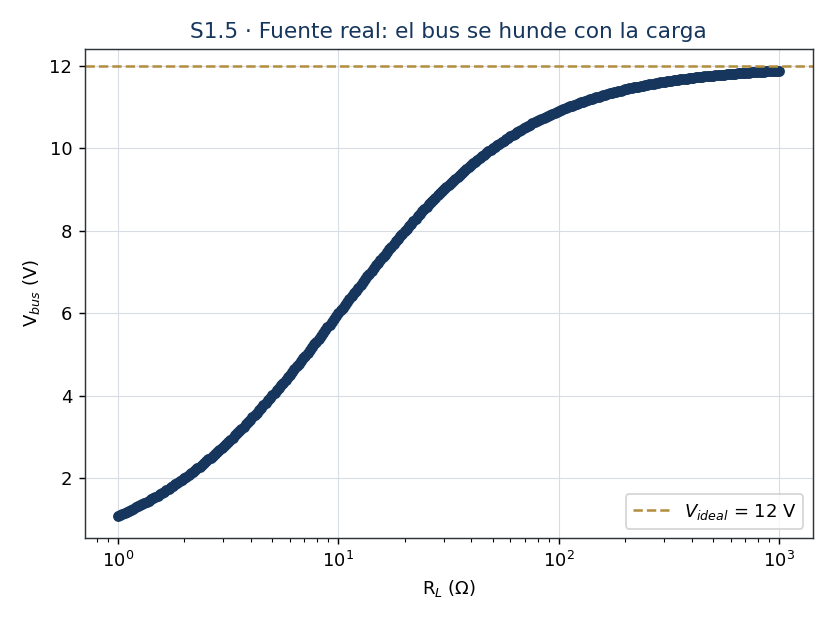
\includegraphics[width=0.78\textwidth]{figs/s15_fuente_real.png}
    \end{center}
    \begin{itemize}
      \item El bus se hunde al aumentar la carga: con $R_L=10\,\Omega$ entrega solo 6 V.
    \end{itemize}
  \end{frame}

  % ---------------------------------------------------------------------
  \begin{frame}{Errores comunes}
  \begin{table}
    \small
    \begin{tabular}{p{0.34\textwidth}p{0.30\textwidth}p{0.30\textwidth}}
      \toprule
      Error & Consecuencia & Corrección \\
      \midrule
      Tratar la fuente como ideal siempre & Subestimar caídas del bus & Usar el divisor $R_L/(R_{int}+R_L)$ \\
      Calcular $P_{int}$ con $V_{ideal}$ en vez de la caída real & Potencia errónea & $P_{int} = I^2\,R_{int}$ \\
      No prever el corto & Sobrecalentamiento/fuego & Límite de corriente + fusibles \\
      Armar $R_L = 1\,\Omega$ en protoboard & Corrientes de amperios & Solo simulación \\
      \bottomrule
    \end{tabular}
  \end{table}
\end{frame}

% ---------------------------------------------------------------------
\begin{frame}{Lectura aeroespacial}
  \begin{itemize}
    \item \textbf{Bus de 28 V de aviónica:} la regulación de carga es una especificación
      del bus; el equipo debe operar en el rango aceptado aunque el bus caiga con la carga máxima.
    \item \textbf{Protección:} el dimensionamiento de fusibles y limitadores se hace con
      el peor caso de corriente (KCL de S1.3): una rama en corto no debe tumbar el bus.
    \item \textbf{EPS del satélite:} la batería y el regulador tienen resistencia
      interna; al dimensionar la energía se modela la caída bajo demanda pico.
    \item El \textbf{arnés} añade resistencia en serie: cableado largo + carga pesada
      = caída apreciable (mismo modelo, $R_{int}$ = arnés + fuente).
  \end{itemize}
\end{frame}

% ---------------------------------------------------------------------
\begin{frame}{Preguntas de verificación}
  \begin{enumerate}
    \item ¿Por qué el bus cae cuando la carga exige más corriente?
    \item Con $V_{ideal} = 12$ V y $R_{int} = 10\,\Omega$: ¿qué $V_{bus}$ entrega con $R_L = 100\,\Omega$?
      \uncover<2->{\emph{(\SI{10.91}{\volt}.)}}
    \item ¿Qué disipa la resistencia interna con $R_L = 10\,\Omega$?
      \uncover<3->{\emph{(\SI{3.6}{\watt}: la mitad de la potencia se pierde en la fuente.)}}
    \item ¿Por qué se necesita límite de corriente si el modelo ya ``predice'' la caída?
      \uncover<4->{\emph{(El modelo predice, pero no protege: la disipación interna quema la fuente.)}}
    \item ¿Qué cambia si $R_{int}$ fuera de $1\,\Omega$ en lugar de $10\,\Omega$?
  \end{enumerate}
\end{frame}


\end{document}
